\documentclass{article}

% Language setting
% Replace `english' with e.g. `spanish' to change the document language
\usepackage[english]{babel}

% Set page size and margins
% Replace `letterpaper' with `a4paper' for UK/EU standard size
\usepackage[letterpaper,top=2cm,bottom=2cm,left=3cm,right=3cm,marginparwidth=1.75cm]{geometry}

% Useful packages
\usepackage{amsmath}
\usepackage{graphicx}
\usepackage[colorlinks=true, allcolors=blue]{hyperref}

\title{Big Data Housing market analysis}
\author{You}

\begin{document}
\maketitle



\section{Introduction}
The Romanian housing market has experienced dramatic trends in the last 5 years, with residential prices in major urban hubs like Bucharest and Cluj-Napoca surging by over 40\%. In this vibrant and essential market, it is important that we establish AI models that are able to reliably predict the price of real estate, in order to decide if the price of certain offers is too high or too low.
\textbf{TODO:CONTINUE}
\section{Dataset production}
We have decided to limit our crawling to flats, not houses, that are in Bucharest. This approach allows us to have more homogenous data, facilitating the tasks of our algorithms.
 We set a target of 10000 different samples from 2 websites : \emph{imobiliare.ro} and \emph{storia.ro}. This equal split is able to correct biases related to the platform, but also make sure that we have enough data for the Machine Learning section. In order to obtain all the relevant data from each website, we first notice that all the listings are make available using pagination (e.g. on page 1 there are 10 listing , on page 2 there are 10 listing and so forth). After we gather 10 000 links/listings, each property is analysed using an automated script. On \emph{storia.ro}, there are no rate limits for crawling, so everything could be done in one session, however \emph{imobiliare.ro} imposes limits on crawling, resulting in a process conducted in multiple sessions.

 For each listing, the following relevant attributes were collected:

\begin{itemize}
    \bfseries
    \item URL \texttt{String}
    \item Price \texttt{Int}
    \item Surface \texttt{Float}
    \item Nr. of rooms \texttt{Int}
    \item Floor \texttt{Int}
    \item Max Floor \texttt{Int}
    \item Year built \texttt{Int}
    \item City \texttt{String}
    \item Elevator \texttt{Bool}
    \item Construction Material \texttt{String}
    \item Nr. of bathrooms \texttt{Int}
    \item Latitude \texttt{Float}
    \item Longitude \texttt{Float}
    \item Metro Proximity \texttt{Float}
    \item STB Proximity \texttt{Float}
\end{itemize}
 
 Metro Proximity represents how close the listing is to the nearest metro station, and STB Proximity how close it was to any other public transit. They were computed using the latitude and the longitude of the listing, and comparing it to all the latitudes and longitudes of all the  stations.

Furthermore, we also decided to collect how many floors the building has, as there is an inverse relationship between how many floors there are in total and the price.

Each attribute was collected using the specific \texttt{HTML} tag, and also the inner text describing the element as show in Figure ~\ref{fig1}

\begin{figure}
    \centering
    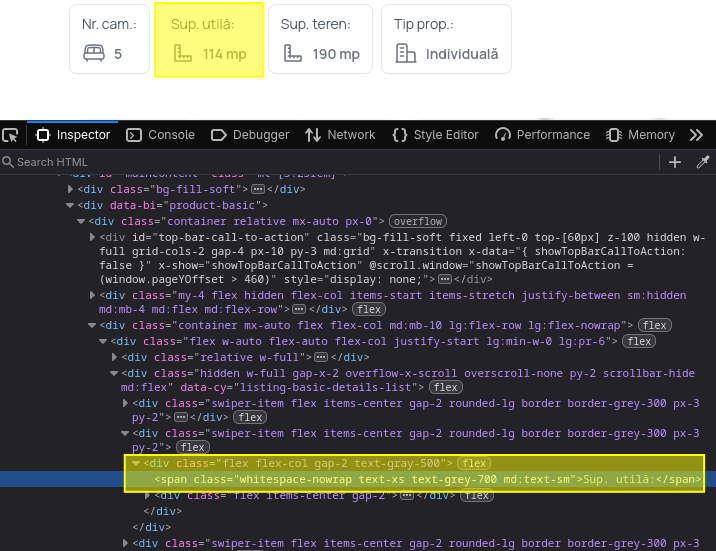
\includegraphics[width=0.5\linewidth]{figure1.png}
    \caption{The highlighted code illustrates that the \texttt{class} tag and the inner \texttt{HTML} text uniquely identify the highlighted website element }
    \label{fig1}
\end{figure}

\section{Dataset description}

\end{document}
